\chapter{Consistency} \label{ch:consistency}

Consistency is a condition where all nodes in a system agree on the current state of the system and see the same data at the same time. In a centralized system, this challenge often becomes more manageable, as decisions that change the state of the system are stored in shared memory between processes. In a distributed system with multiple nodes, each processor has its own private memory and the ability to change the state of the system, so state information must be passed from one node to the next. This can create consistency problems, when nodes become out of sync or somehow do not reflect the current state of the system due to server failures, bandwidth bottlenecks or network topology changes. In this chapter we look at the CAP and PACELC theorems for consistency and replication, and discuss various consistency models used in distributed systems.

\section{The CAP theorem}
The CAP stands for Consistency, Availability and Partition Tolerance, and these are three attributes of a distributed system. The consistency attribute means that if a node has been written to, then if another node is read from, it will return what was just written to the other node. In other terms, if a node is written to it will return the newest version of the data given to any node in the system. The availability attribute promise that when a node is spoken to it will respond, unless that node has failed, the availability attribute allows for failed nodes but in any other case it will respond. The partition tolerance means that when the network is partitioned then whatever other promises are made about the system, it will still keep those promises. A network is partitioned, when messages can't flow from one machine to another. This might happen if you have two different data centers and the connection between the two is separated. On Figure \ref{fig:cap_triangle} a simplified version of the theorem can be seen, as well as examples of which attributes, some  of the more known databases, support.

\begin{figure}[h!]
	\centering
	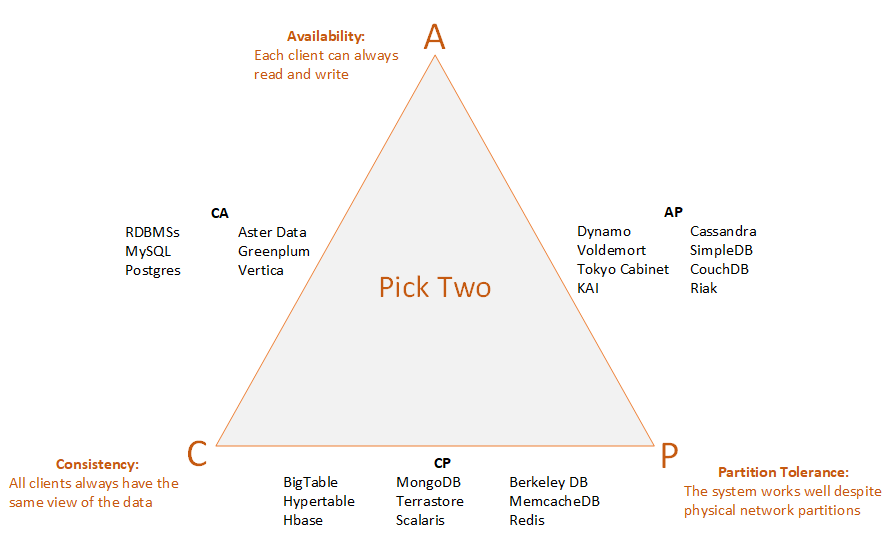
\includegraphics[width=0.61\linewidth]{consistency/fig/cap_triangle.png}
	\caption{CAP theorem triangle, with examples of database attribute support.}
	\label{fig:cap_triangle}
\end{figure}

The CAP theorem says, that a distributed system, can only have up to two of these attributes fulfilled at a given time. On Figure \ref{fig:cap_proof} the proof, of the three scenarios, is illustrated. Case A; there is a partition between Node A and Node B. The new data that is send to Node A can not be read from Node B, therefor the system is not consistent. Case B; there is a partition between Node A and Node B. Since the new data can not be send between the nodes and the system won't send old data Node B won't respond to the read request, this makes the system not available. Case C; there is no partition between the nodes, therefor the system is not partition tolerant.

\begin{figure}[h!]
	\centering
	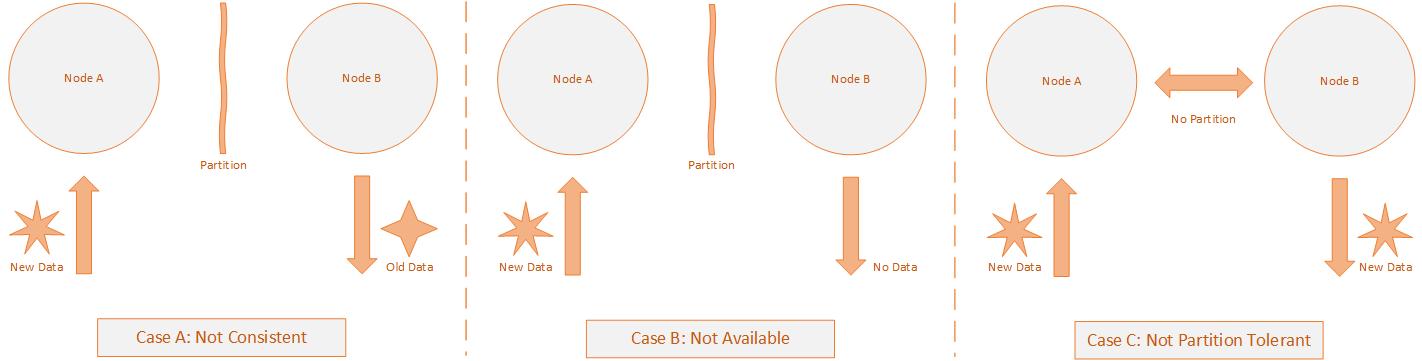
\includegraphics[width=0.9\linewidth]{consistency/fig/cap_proof.png}
	\caption{CAP theorem three possible outcomes.}
	\label{fig:cap_proof}
\end{figure}


\section{PACELC}
The PACELC theorem is a addition to the CAP theorem. This addition tries to describe a more full picture where that even in the absence of partitions there's a tradeoff between consistency and latency. In CAP, one must choose between high availability and consistency. This leaves no option for mission-critical applications but to sacrifice consistency because high availability is a given. This logic is not right because the P in CAP is a mix of \textit{partition tolerance} and a \textit{actual network partition}. Therefore it is wrong to assume the systems that reduce consistency in the absence of any partitions are doing it because of CAP. PACELC handles the cases when a network partition have or not happened.

\noindent The theorem states: If there is a partition \textbf{P}, how does the system trade off availability \textbf{A} and consistency \textbf{C}. Else, when the system is running normally in
the absence of partitions, how does the system trade off latency \textbf{L}
and consistency \textbf{C}\footnote{Appendix 1 - Fischer\_DIPS\_S05\_Synchronization\_Slides, p.~13}

\noindent Apache's \textbf{Cassandra} database system is a PA/EL system. If a partition happens, it will give up consistency for availability, and during normal operation gives up consistency for lower latency. Google's \textbf{BigTable}
follows ACID\footnote{ACID (Atomicity, Consistency, Isolation, Durability) is a set of properties of database transactions intended to guarantee validity even in the event of errors, power failures, etc.} hence PC/EC. It will refuse to give up consistency and pay the price in terms availability and latency costs to achieve it. \textbf{MongoDB} can be classified as a PA/EC system. In the default configuration, the system guarantees reads and writes to be consistent.\footnote{\cite[p.~42]{Abadi2012}}
When a system have a network partition happen to it there is a few options for replication the data.
\begin{enumerate}
	
	\item Data updates sent to all replicas at the same time.
	\begin{enumerate}
		\item Using a preprocessing layer gives us consistency but increased latency.
		\item Not using a preprocessing layer will decrease latency but can only offer eventual consistency.
	\end{enumerate}
	\item Data updates sent to an agreed-upon location first
	\begin{enumerate}
		\item Synchronous the master node waits until updates made it to the replicas. Therefor gaining consistency but pays latency.
		\item Asynchronous treats the update as if it were completed before being sent to a replica.
	\end{enumerate}
	\item Data updates sent to an arbitrary location first.
		\begin{enumerate}
		\item Synchronous then the latency problems of (2)(a) are present.
		\item Asynchronous consistency problems same as (1) and (2)(b) are present.
	\end{enumerate}
\end{enumerate}

\begin{table}[H]
	\centering
\begin{tabular}{|c|c|c|c|c|}
	\hline 
	System & A & C & L & C \\ 
	\hline 
	Cassandra & X &  & X &  \\ 
	\hline 
	BigTable &  & X &  & X \\ 
	\hline 
	MongoDB &  & X & X &  \\ 
	\hline 
\end{tabular}
  \caption{This is my one big table} \label{tab:PACELC}
\end{table}

\newpage
\section{Consistency models}

Consistency models are used in distributed systems like shared memory storage, filesystems and databases to amend the issues that distributed write and read access could have to such a system. A consistency model define a given set of rules a operation must follow when accessing the data and can be seen as a contract between a running process (the programmer) and the system. If the process comply with this contract, then memory will be consistent and the output of reading, writing, or updating the memory will be predictable. For example in relational database systems, transactions abide by the ACID principle, where consistency ensures that any transition will bring the database from one valid state to the next and that data should follow a set of rules. Assume a relational database in a cluster that contain row $R_x$ and that this row is replicated to nodes $Node_a$ and $Node_b$. A client $C_i$ then writes $R_x$ on $Node_a$. Subsequently another client $C_j$ reads $R_i$ from $Node_b$. A consistency model has to determine if $C_j$ sees the write from $C_i$ or not.

\noindent Consistency models can be classified as strong or weak. A strong consistency model guarantees that the order and visibility of updates are equivalent to that of a centralized (non-replicated) system with only one process, that is updates are immediately replicated to all nodes. A weak consistency model does not make this guarantee. We will now look at both strong and weak models and consider them for a distributed system:

\noindent \textbf{Linearizability}: A strong consistency model that ensures that all operations appear to have run atomically (in isolation, independent from concurrent processes) in an order that is consistent with the global real-time ordering of operations. If a distributed database follows this model, than it would appear centralized to its clients. No matter how clients execute operations, the result would be the same as if they we executed in some sequential order and these operations appear in their order of executing.

\noindent \textbf{Sequential consistency}: A strong consistency model that mimics the linearizability one, but does not require that two independent operations from different clients respect the real-time ordering of operations in a system. With this model, operations can be re-ordered as long as each node observe the ordering consistently. A benefit of the two strong consistency models is that a client or programmer can replace a centralized system with a distributed one without facing data consistency issues.

\noindent \textbf{Client-centric consistency:} A range of various weak consistency models that makes guarantee to clients (users) of data. It ensures that a client may never see old versions of data, if they have already seen a newer one. This can be implemented with client-side caching, so if the client suddenly connects to a node with old data on it, then the application will present a cached version to the client. Still this may not be the newest version of the data globally, hence the weak consistency predicate.

%%http://www.bailis.org/blog/safety-and-liveness-eventual-consistency-is-not-safe/
%%https://www.allthingsdistributed.com/2008/12/eventually_consistent.html
\noindent \textbf{Eventual consistency}: A weak consistency model that guarantees that if an update has changed the state of one node in a system, after a undefined amount of time all nodes will reflect the same state, if no more values are changed. During this period of time (the inconsistency window) some nodes may be consistent and some may not. The size of this window is determined based on communication delay between nodes, system load and the number of nodes involved in the replication scheme. DNS (Domain Name System) and popular NoSQL datastores like Cassandra and DynamoDB implement a eventual consistency model. Eventual consistency is often refereed to as a liveness property, whereas a stronger model like linearizability is a safety property.

\noindent \textbf{Casual consistency}: A weak consistency model that captures the causal relationships between operations in the system, meaning that an update on a process becomes visible to another process only it has relationship with that process. If the operation on a process $P_i$ influences another write operation on process $P_j$, then these two operations are causally related. After updating $P_i$, it communicates to $P_j$ that a value was updated, and subsequent access by $P_j$ will return the updated value and writes will supersede it.

\noindent To recap, which model you choose is a tradeoff between availability and consistency. A system with high avaliabily may suffer from weak consistency and wise versa. We saw this in the PACELC theorem.
